\section{Redis}
\subsection{Charakterisierung}
Redis ist ein Open Source, In-Memory Datenbanksystem, das als vorallem als Datenbank, Cache und Message Broker verwendet werden kann.\\
Redis ist BSD lizenziert und stellt somit keine Anforderungen an die Weiterverteilung der Software.\\
Der Name Redis entstand als Abkürzung für remote dictionary server.\\
Entwickelt wurde Redis 2009 von Salvatore Sanfilippo in C und gehört mitlerweile zu VMWware. Die aktuelle Version (Stand 5. November 2019) ist 5.0.5, wobei die aktuelle LTS Version 3.2.11 ist.
Redis ist single-threaded und lässt sich einfach replizieren.

\subsubsection{Platformen, welche Redis verwenden}
Redis erfreut sich grosser Beliebtheit und ist laut DB-Engines.com die verbreitetste Key-Value Datenbank.
Einige der grossen Kunden sind etwa Twitter (Real-Time Delivery), Github (Speicherung von Routing Information) und StackOverflow (2-Level Cache).\\
Mehr Infos unter: https://redis.io/topics/whos-using-redis
\subsection{Installation}
Redis lässt sich leicht als tar.gz gerunterladen und installieren:
\begin{lstlisting}[language=bash]
wget http://download.redis.io/redis-stable.tar.gz
tar xvzf redis-stable.tar.gz
cd redis-stable
make
make install
\end{lstlisting}
Falls gewünscht lässt sich Redis auch mittels Docker installieren.\\
Mehr Infos unter: https://redis.io/topics/quickstart
\clearpage
\subsection{Datentypen}
Redis unterstützt die folgenden Datentypen:
\begin{table}[H]
	\begin{tabular}{|p{3cm}|p{12.7cm}|}
		\hline
		\rowcolor{black}
		\textcolor{white}{\textbf{Typ}} &
		\textcolor{white}{\textbf{Beschreibung}}\\
		
		String & Eine beliebige Zeichenfolge\\ 
		\hline
		List & Entspricht einem Array, die Elemente werden über einen positiven, ganzzahligen, null-basierten Index angesprochen \\
		\hline 
		Hash & Entspricht einem assoziativem Array, die Elemente bestehen hier wiederum aus Schlüssel-Werten Paaren.\\
		\hline 
		Set & Wie List, jedoch kann jedes Element nur einmal vorkommen darf.\\
		\hline 
		Sorted Set & Entspricht einem Set, nur dass zusätzlich der Index des Elements explizit mit angegeben wird.\\
		\hline 
		Bitmaps & Speicherung von Bits\\
		\hline 
		HyperLogLogs & Probabilistische Datenstruktur, mit der sich die Kardinalität einer Datenmenge sehr speichereffizient bestimmen lässt\\
		\hline
	\end{tabular}
\end{table}
Mehr Infos unter: https://redis.io/topics/data-types
\subsection{Abfragesprache}
Für String lässt sich ein Speichern und Abrufen mit get und set erreichen (alle Beispiele mit Python Redis):
\begin{lstlisting}[language=python]
import redis
r = redis.Redis()
r.set("msg:hello", "Hello Redis!!!")
msg = r.get("msg:hello")
# prints b'Hello Redis!!!'
\end{lstlisting}

Für jeden Datentyp gibt es solche Schreib- und Lesebefehle. Zudem gibt es diverse weitere Befehle (z.B. zum Zählen der Elemente). Nachfolgend ein Beispiel für ein Set:
\begin{lstlisting}[language=python]
mountainSet = "Berge"
# Add elements to the Redis set
r.sadd(mountainSet, "Eiger")
r.sadd(mountainSet, "Moench")
r.sadd(mountainSet, "Jungfrau")

print("Anzahl Elmente: ")
print(r.scard(mountainSet))
print(r.smembers(mountainSet))
# prints Anzahl Elmente: 3 {b'Eiger', b'Moench', b'Jungfrau'}
\end{lstlisting}
Eine Liste aller Abfragen findet sich hier: https://www.cheatography.com/tasjaevan/cheat-sheets/redis/
\subsubsection{Transaktionen}
Eine Transaktion in Redis besteht aus einem Block von Befehlen, die zwischen MULTI und EXEC (oder DISCARD für Rollback) platziert werden. Sobald ein MULTI gefunden wurde, werden die Befehle auf dieser Verbindung nicht ausgeführt - sie stehen in der Warteschlange (und der Anrufer erhält die Antwort QUEUED). Wenn eine EXEC angetroffen wird, werden sie alle in einer einzigen Transaktion angewendet (d.h. ohne dass andere Verbindungen Zeit zwischen den Operationen erhalten). Wenn anstelle von EXEC eine DISCARD gesehen wird, wird alles weggeworfen. Da die Befehle innerhalb der Transaktion in der Warteschlange stehen, können Sie innerhalb der Transaktion keine Entscheidungen treffen.

Sämtliche Informationen dazu finden sich hier: https://redis.io/topics/transactions

\subsection{Benchmarks}
Redis bietet das Dienstprogramm redis-benchmark, das laufend Befehle von Clients simuliert und gleichzeitig Gesamtabfragen sendet. Damit kann die Performance von Redis getestet und visualisiert werden.
Anleitungen und Beispiele dazu finden sich hier: https://redis.io/topics/benchmarks

\subsection{Persistenz}
Redis bietet generell zwei Varianten der sicheren Datenspeicherung:

RDB (Snapshots): Zu bestimmten Zeitpunkten (z.B. jede volle Stunde) wird eine vollständige Kopie der im Speicher befindlichen Daten erstellt. Wenn z.B. zwischen zwei Snapshots die Stromversorgung verlieren geht, gehen die Daten aus der Zeit zwischen dem letzten Snapshot und dem Crash verloren. 

AOF: Logt jede vom Server empfangene Schreiboperation und führt diese beim Serverstart erneut ab zur Rekonstruktion des ursprünglichen Datensatzes.

Grundsätzlich lassen sich RDB und AOF einzel aktiviren. Somit wäre auch keine Persistenz möglich, in dem beides deaktiviert wird. Die beste Persistenz wird erreicht, in dem beides aktiviert wird. Grundsätzlich handelt es sich hierbei um eine Frage zwischen Datensicherheit und Leistung.\\
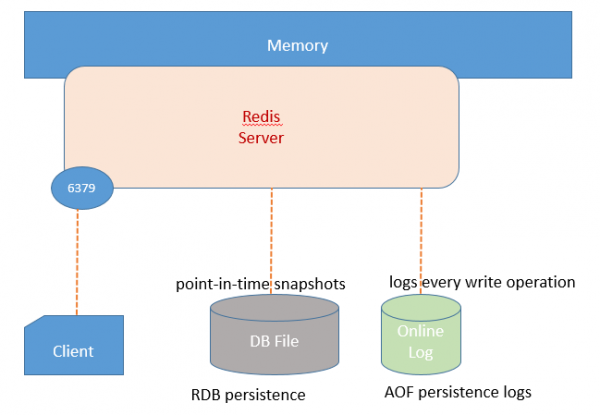
\includegraphics[width=70mm]{media/redis.png}\\[10mm]	
Weitere Vor- und Nachteile finden sich hier: https://redis.io/topics/persistence
\subsection{Replikation}
Typisches Design\\
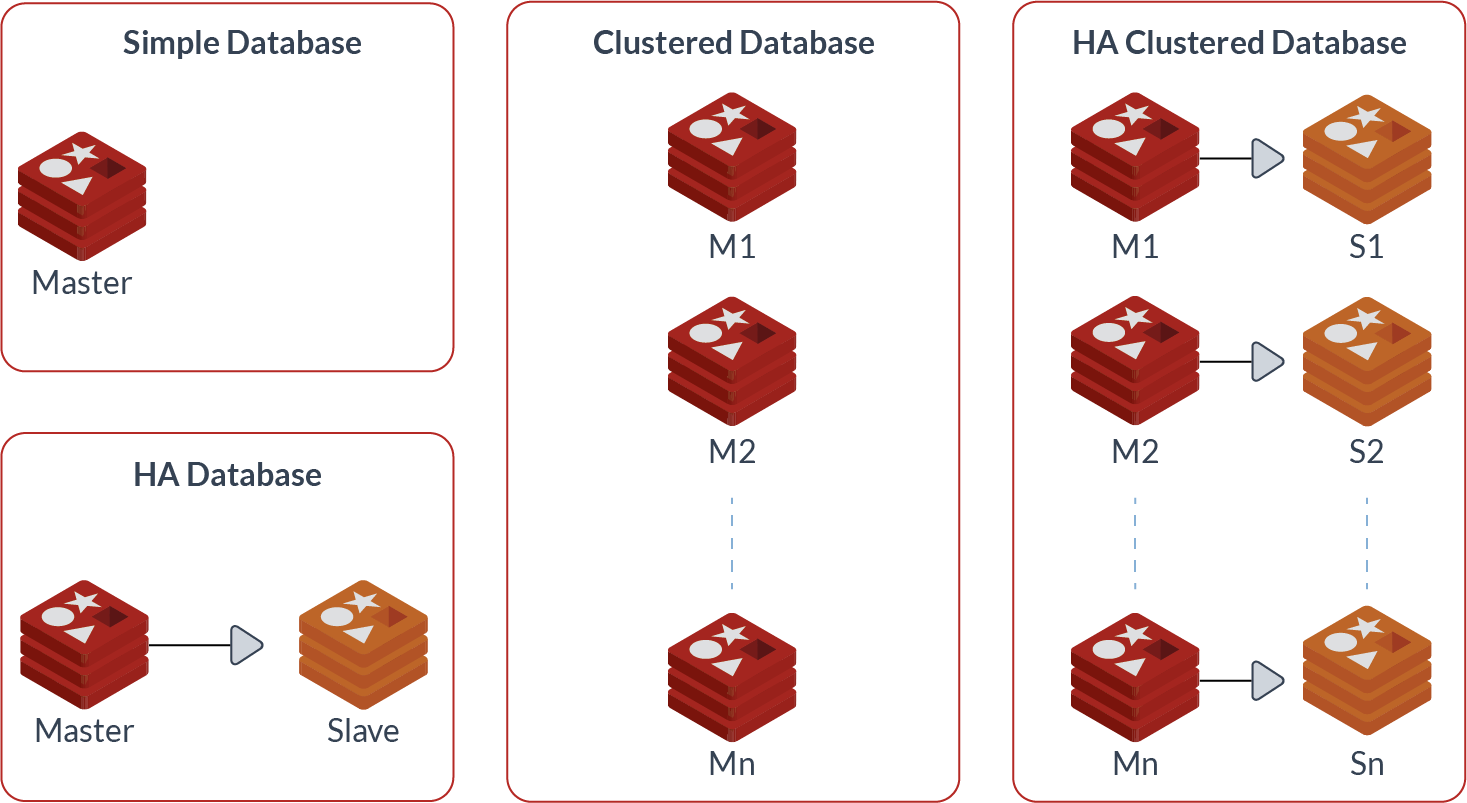
\includegraphics[width=100mm]{media/diagram-cluster-architecture.png}\\[10mm]	
Verteilte Datenhaltung, Skalierbarkeit, Protokolle, Architektur
https://redis.io/topics/replication
\subsection{Optimierungsmöglichkeiten}
https://redis.io/topics/memory-optimization
\subsection{GUI}
https://redislabs.com/blog/so-youre-looking-for-the-redis-gui/
\subsection{API}
https://redis.io/topics/modules-intro\\
mit Demo
\subsection{Massenload}
https://redis.io/topics/mass-insert

\clearpage
\section{Ressourcen}
https://en.wikipedia.org/wiki/Key-value\_database\\
https://db-engines.com/de/ranking/key-value+store\\
https://www.aerospike.com/what-is-a-key-value-store/\\
https://www.ionos.de/digitalguide/hosting/hosting-technik/key-value-store/\\
https://redis.io/\\
https://redislabs.com\\
https://www.pipperr.de/dokuwiki/doku.php?id=nosql:redis\_overview\\
https://wikipedia.org/wiki/Redis\\